\subsection{Merkle Tree}
Merkle hash trees are a class of hash-based binary or multinomial trees where the value on the leaf node is usually the hash of the data block, while the value on the non-leaf node is the hash of the combined result of all the children of that node.
A data integrity audit scheme based on a Merkle tree and blockchain is a method used to verify the integrity and authenticity of data stored on a blockchain.
\begin{figure}[H]
    \centering
    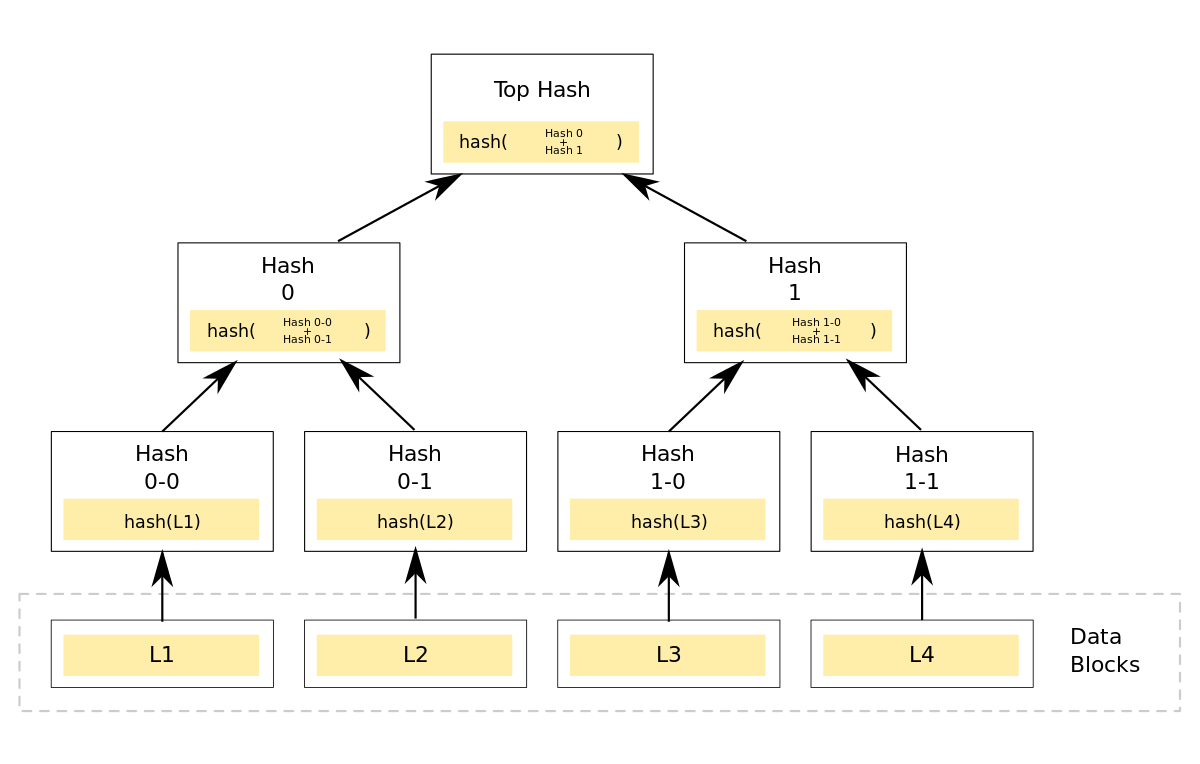
\includegraphics[scale=0.4]{figures/Sparse Merkle Tree.png}
    \caption{Merkle Tree}
 
\end{figure}